\chapter{Background} \label{chap:background}
\section{Schrödinger's equation}
	The most fundamental equation for closed nonrelativistic quantum system is the Schrödinger equation \cite{Nielsen2010-xd} 
	\begin{equation}
		\label{eq:schroedinger}
		-\frac{\hbar^2}{2m}\Delta\Psi(\vec{r},t)+V(\vec{r})\Psi(\vec{r},t)=i\hbar\frac{\partial}{\partial t}\Psi(\vec{r},t),
	\end{equation}
	where $\Delta$ denotes the Laplace-operator and $\hbar$ the reduced Planck constant.
	It assigns wave functions $\Psi$ to a particle with mass $m$ in a real potential $V(\vec{r})$ and describes it's time evolution.
	By making the product ansatz $\Psi(\vec{r},t)=\psi(\vec{r})\Chi(t)$ and after separating variables, 
	\begin{equation}
		\label{eq:schroedinger_productansatz}
		-\frac{\hbar^2}{2m}\frac{1}{\psi(\vec{r})}\Delta\psi(\vec{r})+V(\vec{r})=E=i\hbar\frac{1}{\Chi(t)}\frac{\partial}{\partial t}\Chi(t),
	\end{equation}
	the stationary Schrödinger equation is obtained:
	\begin{equation}
		\label{eq:stat_schroedinger}
		-\frac{\hbar^2}{2m}\Delta\psi(\vec{r})+V(\vec{r})\psi(\vec{r})=E\psi(\vec{r})
	\end{equation}
	For a particle in one dimension, the stationary Schrödinger equation can be written as
	\begin{equation}
		\label{eq:1d_schroedinger}
		-\frac{\hbar^2}{2m}\frac{\partial^2}{\partial x^2}\psi(x)+V(x)\psi(x)=E\psi(x).
	\end{equation}
	By checking the units of the equation, it becomes clear, that regardless of the units of $\psi$, $E$ is a scalar and has the dimension \textit{Energy}.
  \begin{equation}
		\label{eq:1d_schroedinger_units_1}
    \left[-\frac{\hbar^2}{2m}\frac{\partial^2}{\partial x^2}\psi(x)\right]+\left[V(x)\psi(x)\right]=\left[E\psi(x)\right] 
  \end{equation}
  \begin{equation}
		\label{eq:1d_schroedinger_units_2}
    \frac{J^2s^2}{kg}\left[\frac{\partial^2}{\partial x^2}\psi(x)\right]+\left[V(x)\right]\left[\psi(x)\right]=\left[E\right]\left[\psi(x)\right]
  \end{equation}
  \begin{equation}
		\label{eq:1d_schroedinger_units_3}
    Jm^2\frac{1}{m^2}\left[\psi(x)\right]+J\left[\psi(x)\right]=\left[E\right]\left[\psi(x)\right]
  \end{equation}
  \begin{equation}
		\label{eq:1d_schroedinger_units_4}
    J=\left[E\right]
  \end{equation}
	To further simplify the equation, an operator $H$ can be defined: 
	\begin{equation}
		\label{eq:hamilton_operator}
		H = -\frac{\hbar^2}{2m}\frac{\partial^2}{\partial x^2}+V(x)
	\end{equation}
	It is called Hamilton-operator or Hamiltonian and it depends on $V(x)$, therefore it is different for each physical system. The Schrödinger equation now simplifies to
	\begin{equation}
		\label{eq:schroedinger_with_hamilton}
		H\psi(x) = E\psi(x).
	\end{equation}
	\subsection{Particle in a box} \label{sec:particle_in_a_box}
		One simple one-dimensional problem to give an intuition for the Schrödinger equation is a one-dimensional particle trapped between two infinitely large potential barriers.
		\begin{equation}
			\label{eq:box_potential}
			V(x)=
			\left\{
        		\begin{array}{ll}
            		0 & \quad 0 < x < L \\
            		\infty & \quad \text{otherwise}
        		\end{array}
    		\right.
		\end{equation}
		The resulting differential equation can easily be solved by making an exponential Ansatz 
		\begin{equation}
			\label{eq:box_ansatz}
			\psi(x)=\left\{
				\begin{array}{ll}
					Ae^{ikx}+Be^{-ikx} & \quad 0 < x < L \\
					0 & \quad \text{otherwise}
				\end{array}
			\right.
		\end{equation}
		and demanding continuity of the wave function
		\begin{equation}
			\label{eq:box_boundary_condition}
			\psi(0)=\psi(L)=0.
		\end{equation}
		By applying the boundary conditions and Euler's formula \cite{Riley2006-uk}, $k$ can be found and inserted into the wave function:
		\begin{equation}
			\label{eq:box_unnormalized_wavefunction}
			\psi_n(x)=Nsin\left(\frac{n\pi}{L}x\right), \quad n \in \mathbb{Z}, \quad N \in \mathbb{C}
		\end{equation}
		Because the wave function itself can be complex-valued and does not directly correspond to measurable quantities, squaring its magnitude ensures a real, non-negative value that can be normalized to represent the probability distribution of finding a particle in a given state or position.
		In this case, normalizing the wave function
		\begin{equation}
			\label{eq:normalize_condition}
			\int_{-\infty}^{\infty}\abs{\psi(x)}^2dx=1,
		\end{equation}
		yields $N$ which is then inserted into the wave function
		\begin{equation}
			\label{eq:box_normalized_wavefunction}
			\psi_n(x)=\sqrt{\frac{2}{L}}sin\left(\frac{n\pi}{L}x\right).
		\end{equation}
		Technically not $N$ was found but $\abs{N}$. $N$ can have a complex phase, but as this global phase does not affect the probability distribution $\abs{\psi(x)}^2$
		\begin{equation}
			\label{eq:global_phase}
			\abs{e^{i\theta}\psi(x)}^2=\left(e^{i\theta}\psi(x)\right)\left(e^{-i\theta}\psi^*(x)\right)=\abs{\psi(x)}^2,
		\end{equation}
		this global phase is ignored. Plugging the wave function back into the Schrödinger equation (\ref{eq:1d_schroedinger}) yields the energies of each wave function:
		\begin{equation}
			\label{eq:box_eigenenergies}
			E_n=\frac{\hbar^2n^2\pi^2}{2mL^2}
		\end{equation}
		These are not the only solutions to the Schrödinger equation.
		In fact, every linear combination of functions $\psi_n(x)$ is also a solution.
		When constructing a simple example $\Phi(x)=a\psi_1(x)+b\psi_2(x)$, it becomes clear, that this solution cannot be assigned a constant energy.
		A particle with this wave function is in superposition. Only when measuring the energy of the particle the wave function collapses into either $\psi_1(x)$ or $\psi_2(x)$ with a probability based on the value of the coefficients $a$ and $b$ \cite{Sakurai2020-lj}.
		The functions $\psi_n(x)$ are special in the sense that they have well defined energies associated with them.
		These functions are called eigenstates or eigenfunctions of the system. The energies $E_n$ are called eigenenergies.
\section{The Postulates of Quantum Mechanics} \label{sec:postulates}
  While the previous section aims to provide an initial intuition for quantum mechanics, this section aims to provide a more rigorous framework to describe quantum systems. The postulates of quantum mechanics establish the connection between the physical world and the mathematical formalism of the theory \cite{Nielsen2010-xd}.
	\begin{postulatebox}
		\begin{postulate}
			\label{post:qm_1}
			Associated to any isolated physical system is a complex vector space with inner product (that is, a Hilbertspace) known as the state space of the system. The system is completely described by its state vector, which is a unit vector in the system's state space.
		\end{postulate}
	\end{postulatebox}
	The wavefunction $\psi_n(\vec{r})$ is now represented as an abstract state vectore $\ket{\psi}$ that lives in an $N$-dimensional Hilbertspace $\mathcal{H}$.
	The inner product of that Hilbertspace \cite{Jackson2013-lm} is defined as
	\begin{equation}
		\label{eq:hilbertspace_inner_product_definition}
		\braket{\phi}{\psi}=\int_{\mathbb{R}^3}\phi(\vec{r})^*\psi(\vec{r})d\vec{r}.
	\end{equation}
	It follows, that if and only if the wavefunctions $\phi(\vec{r})$ and $\psi(\vec{r})$ are orthogonal to each other, the inner product $\braket{\phi}{\psi}=0$. Also, for the state vector $\ket{\psi}$ to be a unit vector, it has to be normalized such that
	\begin{equation}
		\label{eq:psi_normalize}
		\braket{\psi}{\psi}=1.
	\end{equation}
	The number of dimensions $N$ of the Hilbertspace $\mathcal{H}$ equals the number of eigenstates of the system. In the example of a particle in a box, discussed in Section \ref{sec:particle_in_a_box}, $N$ would be countable infinite.
	\begin{postulatebox}
		\begin{postulate}
			\label{post:qm_2}
			The evolution of a closed quantum system is described by a Unitary transformation. That is, the state $\ket{\psi}$ of the system at time $t_1$ is related to the state $\ket{\psi'}$ of the system at time $t_2$ by a Unitary operator $\hat{U}$ which depends only on the times $t_1$ and $t_2$,
			\begin{equation}
				\label{eq:time_evolution}
				\ket{\psi'}=\hat{U}\ket{\psi}.
			\end{equation}
		\end{postulate}
	\end{postulatebox}
	This postulate describes the time evolution of closed physical systems. An equivalent description of that postulate would be: \textit{The time evolution of the state of a closed quantum system is described by the Schrödinger equation,}
	\begin{equation}
		\label{eq:time_evolution_schroedinger}
		\hat{H}\ket{\psi}=i\hbar\frac{d\ket{\psi}}{dt}.
	\end{equation}
	Equation (\ref{eq:time_evolution_schroedinger}) was alredy introduced in equation (\ref{eq:schroedinger}) with the difference being the description using a state vector $\ket{\psi}$ instead of a wave function in position space and $\hat{H}$ being the Hamilton-operator describing the physical system. In this notation it is independent of the basis. In this thesis, operators written with a hat (e.g., $\hat{A}$) denote basis-independent representations, while those without a hat (e.g., $A$) denote a representation in a specific basis. In the position-basis, $H$ has the form
	\begin{equation}
		\label{eq:hamilton_operator_position_space}
		H=-\frac{\hbar^2}{2m}\Delta + V(\vec{r}),
	\end{equation}
	which is similar to equation (\ref{eq:hamilton_operator}), with the only difference being that it uses three dimensions instead of one. This is not the only representation of the Hamilton-operator. It can also for example be represented in its eigenbasis $\{\ket{\psi_1},\ket{\psi_2},\ket{\psi_3},...,\ket{\psi_N}\}$:
	\begin{equation}
		\label{eq:hamilton_eigenbasis}
		H=\begin{pmatrix}
			E_1 & 0 & 0 & \cdots & 0 \\
			0 & E_2 & 0 & \cdots & 0 \\
			0 & 0 & E_3 & \cdots & 0 \\
			\vdots & \vdots & \vdots & \ddots & \vdots \\
			0 & 0 & 0 & \cdots & E_N
			\end{pmatrix}
	\end{equation}
	where $E_n$ are the eigenenergies of the system, giving the stationary Schrödinger equation
	\begin{equation}
		\label{eq:stationary_schroedinger}
		H\ket{\psi_n}=E_n\ket{\psi_n}.
	\end{equation}
	\begin{postulatebox}
		\begin{postulate}
			\label{post:qm_3}
			Quantum measurements are described by a collection $\hat{M}_m$ of measurement operators. These are operators acting on the state space of the system being measured. The index $m$ refers to the measurement outcomes that may occur in the experiment. If the state of the quantum system is $\ket{\psi}$ immediately before the measurement then the probability that result $m$ occurs is given by
			\begin{equation}
				\label{eq:measurement_probability}
				p(m)=\bra{\psi}\hat{M}_m^\dagger \hat{M}_m\ket{\psi},
			\end{equation}
			and the state of the system after the measurement is
			\begin{equation}
				\label{eq:state_after_measurement}
				\ket{\psi_m}=\frac{\hat{M}_m\ket{\psi}}{\sqrt{\bra{\psi}\hat{M}_m^\dagger \hat{M}_m\ket{\psi}}}
			\end{equation}
			The measurement operators satisfy the completenes equation,
			\begin{equation}
				\label{eq:measurement_completeness}
				\sum_{m}\hat{M}_m^\dagger \hat{M}_m=\hat{\mathbbm{1}}.
			\end{equation}
		\end{postulate}
	\end{postulatebox}
	From equation (\ref{eq:state_after_measurement}) follows, that a measurement alters the state. The statevector $\ket{\psi}$ collapses into one of the possible results $\ket{\psi_m}$ with the probability $p(m)$, while giving the measurement result $m$. For example, if a state $\ket{\psi}$ in a two dimensional Hilbertspace is prepared as
	\begin{equation}
		\label{eq:measurement_example_preparation}
		\ket{\psi}=\frac{1}{\sqrt{2}}\left(\ket{\psi_1}+\ket{\psi_2}\right),
	\end{equation}
	where $\ket{\psi_1}$ and $\ket{\psi_2}$ are eigenstates of the system described by an operator $\hat{A}$ with the distinct eigenvalues $a_1$ and $a_2$, the measurement operators are given by
	\begin{equation}
		\label{eq:example_measurement_operator_1}
		\hat{M}_{a_1}=\ketbra{\psi_1}{\psi_1},
	\end{equation}
	\begin{equation}
		\label{eq:example_measurement_operator_2}
		\hat{M}_{a_2}=\ketbra{\psi_2}{\psi_2}.
	\end{equation}
	This definition satisfies the completeness equation (\ref{eq:measurement_completeness}), as $\ket{\psi_1}$ and $\ket{\psi_2}$ form a complete orthonormal system
	\begin{equation}
		\label{eq:cons_completeness}
		\sum_{i}\ketbra{\psi_i}{\psi_i}=\hat{\mathbbm{1}}.
	\end{equation}
	Using equation (\ref{eq:measurement_probability}), a general expression for the probability $p(a_i)$ can be found:
	\begin{equation}
		\label{eq:measurement_probability_a}
		p(a_i)=\abs{\braket{\psi_i}{\psi}}^2
	\end{equation}
	In the given example, the probability of measuring $a_1$ results in $\frac{1}{2}$ and the state immediately after the measurement - if $a_1$ is the outcome of the measurement - becomes $\ket{\psi_1}$. Equation (\ref{eq:measurement_completeness}) also ensures, that the probabilities $p(m)$ of all possible measurement outcomes add to $1$:
	\begin{equation}
		\label{eq:measurement_probability_sum}
		\sum_{m}p(m)=\sum_{m}\bra{\psi}\hat{M}_m^\dagger \hat{M}_m\ket{\psi}=\bra{\psi}\sum_{m}\hat{M}_m^\dagger\hat{M}_m\ket{\psi}=\braket{\psi}{\psi}\overset{\eqref{eq:psi_normalize}}{=}1
	\end{equation}
	\begin{postulatebox}
		\begin{postulate}
			\label{post:qm_4}
			The state space of a composite physical system is the tensor product of the state spaces of the component physical systems. Moreover, iff there are independent systems numbered $1$ through $n$, and system number $i$ is prepared in the state $\ket{\psi_i}$, then the joint state of the total system is $\ket{\psi_1}\otimes\ket{\psi_2}\otimes ... \otimes\ket{\psi_n}$.
		\end{postulate}
	\end{postulatebox}
	This postulate provides the mathematical framework to describe composite systems, which play a crucial role in quantum entanglement and in the description of quantum circuits discussed later in this thesis.
\section{Qubits}
	A quantum bit (qubit) is the basic building block of quantum information processing \cite{Aeschbacher2020-tr}.
	It describes a physical system that has two distinctly measurable eigenstates, for example Spin-\sfrac{1}{2} particles \cite{levy2002universal}.
	Using the notation
	\begin{equation}
		\label{eq:rename_statevector}
		\ket{\psi_n} \equiv \ket{n},
	\end{equation}
	these eigenstates are called $\ket{0}$ and $\ket{1}$. That means the qubit lives in a two dimensional Hilbertspace with the basis $\{\ket{0},\ket{1}\}$. This basis is also called computational basis. The state of the qubit can then be represented by a linear combination of the basis vectors:
	\begin{equation}
		\label{eq:qubit_superposition}
		\ket{\psi}=a\ket{0}+b\ket{1} \quad a,b \in \mathbb{C}
	\end{equation}
	From the normalization, a relationship for $a$ and $b$ follows.
	\begin{equation}
		\label{eq:normalize_condition_qubit}
		\braket{\psi}{\psi}\stackrel{!}{=}1 \quad \Rightarrow \quad \abs{a}^2+\abs{b}^2=1
	\end{equation}
	\subsection{Bloch representation}
		The amplitudes $a$ and $b$ of the qubit can be parameterized by angles $\theta$ and $\phi$ \cite{Desurvire2009-sp}:
		\begin{equation}
			\label{eq:bloch_parameterization}
			\ket{\psi}=cos\left(\frac{\theta}{2}\right)\ket{0}+e^{i\phi}sin\left(\frac{\theta}{2}\right)\ket{1}.
		\end{equation}
		Now the state can be visualized as a unit vector with angles $\theta$ and $\phi$.
		Two different states are visualized in Figure \ref{fig:bloch_qubits}.
		\begin{figure}[H]
			\centering
			\begin{subfigure}{.35\textwidth}
				\centering
				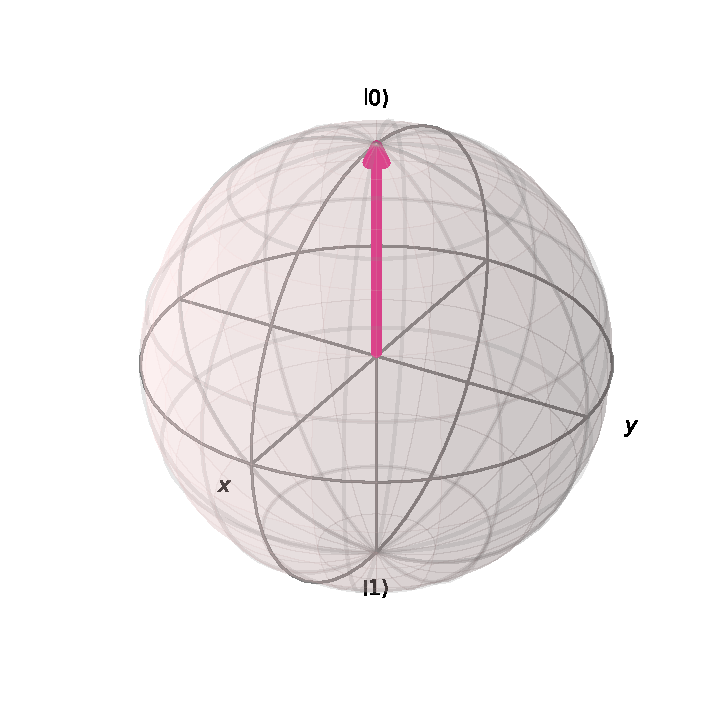
\includegraphics[width=0.95\linewidth]{figures/bloch_0.pdf}
				\caption{$\ket{\psi}=\ket{0}$}
			\end{subfigure}%
			\begin{subfigure}{.35\textwidth}
				\centering
				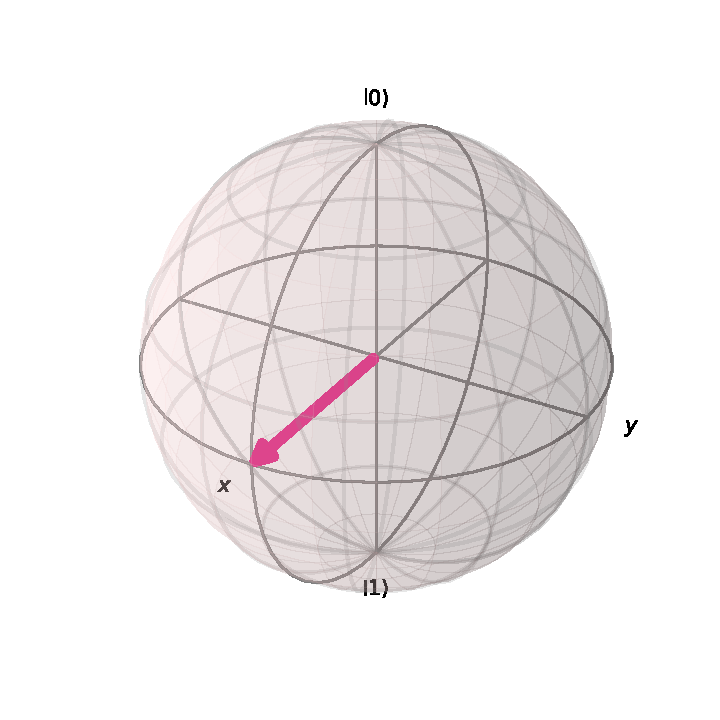
\includegraphics[width=0.95\linewidth]{figures/bloch_superposition.pdf}
				\caption{$\ket{\psi}=\frac{1}{\sqrt{2}}(\ket{0}+\ket{1})$}
			\end{subfigure}
			\caption{Two different qubit states visualized as bloch vectors. (a) has a probability of 100\% to be in the state $\ket{0}$, (b) has a 50\% chance to be either in the state $\ket{0}$ or $\ket{1}$. These visuals were generated using Qiskit \cite{qiskit2024}. The source code for this figure can be found in Listing \ref{lst:bloch_source}}
			\label{fig:bloch_qubits}
		\end{figure}
\section{Entanglement} \label{sec:entanglement}
	With the help of postulate \ref{post:qm_4}, as discussed in section \ref{sec:postulates}, two qubits
	\begin{equation}
		\label{eq:qubit_psi}
		\ket{\psi}=a\ket{0}+b\ket{1}
	\end{equation}
	\begin{equation}
		\label{eq:qubit_phi}
		\ket{\phi}=c\ket{0}+b\ket{1}
	\end{equation}
	can be described together in a composite system by joining their respective Hilbertspaces:
	\begin{equation}
		\label{eq:qubit_composite_hilbertspace}
		\mathcal{H}_{\psi\phi}=\mathcal{H}_\psi\otimes\mathcal{H}_\phi.
	\end{equation}
	Using the notation
	\begin{equation}
		\ket{nm}\equiv\ket{n}\otimes\ket{m},
	\end{equation}
	the computational product basis for this new Hilbertspace is $\{\ket{00},\ket{01},\ket{10},\ket{11}\}$, allowing a state in this Hilbertspace to be in the form of
	\begin{equation}
		\label{eq:allowed_states_in_composite_two_qubits}
		\alpha\ket{00}+\beta\ket{01}+\gamma\ket{10}+\delta\ket{11}.
	\end{equation}
	Postulate \ref{post:qm_4} also states, that the joint state of the two qubits equals to $\ket{\psi}\otimes\ket{\phi}$, which, when considering that both qubits must be normalized, only has two degrees of freedom, while a state prepared in the new Hilbertspace has three degrees of freedom. That means there are states in a composite system, that cannot be realized by only manipulating the qubits on its own. Such a state cannot be seperated into two qubits anymore and is called an entangled state \cite{Nielsen2010-xd}. In this state, the qubits are correlated to each other. The measurement of one qubit determines the measurement outcome of the other qubit. One example of such a preparation would be 
	\begin{equation}
		\label{eq:two_qubit_entangled}
		\ket{\Psi}=\frac{1}{\sqrt{2}}\left(\ket{01}+\ket{10}\right).
	\end{equation}
	For this state, there do not exist two qubit states $\ket{\psi}$ and $\ket{\phi}$ such that $\ket{\psi}\otimes \ket{\phi}=\ket{\Psi}$. Another way of thinking about the state $\ket{\Psi}$ is, that if qubit $\ket{\psi}$ is measured and yields the result $\ket{0}$ the only possible outcome when measuring qubit $\ket{\phi}$ in the same basis is $\ket{1}$. The qubits are dependent on each other.